% -*- coding: utf-8 -*-
%%
%%  本模板可以使用以下两种方式编译:
%%     1. PDFLaTeX
%%     2. XeLaTeX [推荐]
%%  注意:
%%    1. 在改变编译方式前应先删除 *.toc 和 *.aux 文件,
%%       因为不同编译方式产生的辅助文件格式可能并不相同。

\documentclass{cumcmart}
% \documentclass[nocover]{cumcmart}%%%切换到无封面的版本,有些区域不允许前面的承诺页用pdf格式,可以用此去掉。



\begin{document}

\xuanti{测试一}
%\school命令用于在承诺书上显示学校名称。按要求,此处应填写全称
\school{长江大学}
%以下命令分别显示队员及指导教师姓名
\numbers{2017015}%参赛报名号
\authorone{孔庆亮}
\authortwo{陈梓欣}
\authorthree{王张弛}
\advisor{数模指导组}

%\theyear{2017}
% \theday{20}%填写当月的具体日期

\title{公交车调度}
\maketitle
% 摘要
\begin{cnabstract}%此处没有采用sbstract命名,是为了将来如果要加入英文摘要时扩展的方便
本题的数据有一条线路在某一天的上下行中的所有站上下车人数的采集表,让我们确定一个便于操作的全天(工作日)的公交车调度方案。表格数据是离散的,想要使用数据相当不容易,我们使用MATLAB对表格数据进行初步的处理,得到每个时间段、位于每个站点公交车载有的乘客数量,对每个时间段可以寻找到每个时间段的最大载客量,将其看作均匀分布,即可采用三次样条插值法得出最大载客量的连续分布;对这条连续曲线进行分析:利用最大载客量的平均值,可以得到上行方向上的早高峰是$6:00$到$9:00$,下行方向的早高峰是$7:00$到$10:00$;利用MATLAB令发车间隔$t$从十不断减少一,使最大载客量插值线$f(t)$在每个时间段的发车间隔$\Delta t$的变化不超过$120\%$的满载率,利用搜索算法,可以求得不超过$120\%$满载率的在每个时段都最大的发车间隔,从而确定发车时间表,

\cnkeywords{三次样条插值、最优化搜索}
\end{cnabstract}

\newpage
% \tableofcontents \newpage%增加目录,要不要都可以。不想要的话,就在本行前加“%”(英文的百分号)


\section{问题重述}
为了完善城市交通,改善居民出行状况,提高公交公司的经济与社会利益。基于某条公交路线客流调查和运营资料的数据,设计一个在这条线路上便于操作的全天公交车调度方案,包括两个起点站的发车时刻表;一共需要多少辆车;这个方案以怎样的程度照顾到了乘客和公交公司双方的利益,并把这个调度问题抽象成一个明确、完整的数学模型。

\section{建模分析}

\subsection{问题分析}

题中所给数据统计了一个工作日两个运行方向各站上下车的乘客数量,我们将对这组数据进行具体的分析处理,得到每一时间段所有公交车在某两个站点之间的累计人数,由此初步确定该时间段首发站要派出的公交车数量的大体范围。
%   图片
%   \begin{figure}
%   \centering
%   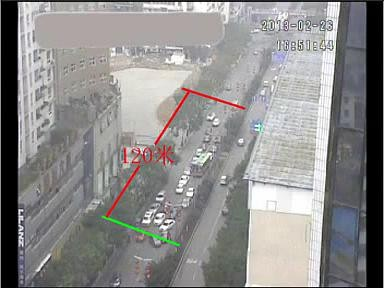
\includegraphics[width=.6\textwidth]{fig1}
%   \caption{发生事故时车流饱和状态图示}
%   \end{figure}

\subsection{模型假设}

\begin{enumerate}
\item 首发站都在五点钟发第一班车;
\item 所有的公交车全程匀速行驶;
\item 公交车上乘客数量的变化,不会影响公交车的速度;
\item 假设表上所给数据能反映该段线路上的日常客流量;
\item 公交车到达终点站时,所有的乘客都会下车;
\item 乘客上行或是下行,无论经过几个站,车票价一定;
\item 公交车会按调度表准时到站和出站;
\item 公交车匀速行驶,不会出现故障,忽略公交车的停站时间
\item 每辆车经过各个车站时不会留有乘客。


\end{enumerate}

\definition  \textbf{最大载客量} \space 每一时间段载客量的最大值。

\subsection{记号说明}
\begin{table}[!htbp]
    \centering
    \begin{tabular}{cl}
    \toprule
    \multicolumn{2}{c}{\large 模型记号说明}\\
    \midrule
    ${p_{max}}$ &  最大载客量 \\
    ${T}$       &  公交车走完全程所花的时间 \\
    ${m_i}$     &  第i时间段首站A13发配的车量 \\
    ${n_i}$     &  第i时间段首站A0发配的车量  \\
    ${a_i}$     &  第i时间段首站派出的车量  \\
    ${t_i}$     &  第i时间段的发车间隔  \\
    \bottomrule
    \end{tabular}
    \caption{模型记号说明}
\end{table}

\subsection{建立模型}
由于两条路线的对称性,这两条路线可以按相同的方式处理,因此我们
对问题分析后,我们建立如下目标优化模型:
\[ \max {m_j}\frac{T}{60} + {m_i}\frac{T}{60} \]
    \[ %\begin{equation}
    s.t.
    \left\{  
    \begin{array}{ll}  
    \frac{a_i}{m_i} \leqslant 120 & i = 1,2\ldots18,j = 1,2\ldots13 \text{ or } 14  \\ 
    \Delta t \leqslant & 
        \left\{
        \begin{array}{l}
        10,\text{非高峰时时间段}\\
        5,\text{高峰时间段}\\
        \end{array}
        \right
    \end{array}  
    \right.
    \] %\end{equation} 





\subsection{模型求解和分析}
\subsubsection{模型的求解 }
第一步
通过对本题所给数据的分析,我们将全天的行车时间依照原来的数据按小时分为24段,得出每个时间段原始数据统计的公交车上每两个站点之间的载客量,
第二步
求出载客量的最大值,据此判断出每个时间段首站派出公交车数量的下限。乘客在非高峰期等待的时间一般不超过10分钟,在高峰期等待的时间一般不超过5分钟,从而知晓各个时间段首站派出车量的最小值作为硬性条件处理
第三步
由第二步确定各个时间段发车时间间隔和以及车次后,首先算出首发站到终点站的距离,,进而具体确定发车具体时刻。
\subsubsection{结果分析 }
结果比实际值会偏大

\subsection{模型评价}
没有考虑车次跨时段的情况,每个时间段每站经过的车次数量都是不一样的,而本模型直接忽略了这一点,存在很大的漏洞
每个站经过的车次应该尽可能的细化。
\subsubsection{模型优点}
1)	模型简单、高效



\subsubsection{模型缺点}
1)	 以最大载客量为基准,得出来的车次偏大,对公司是比较不利的。



\subsection{模型改进}
1.考虑跨时段车次,按各站到首战的时间具体考虑各时间段发配车次。

2.考虑乘客等车时间,并把该因素结合到乘客满意度中。

3.按小时分段不一定最合理,可以采用聚类分析将其进一步分类。   
经检验,下行方向上车人数与下车人数不符,可以通过延长某日调查时段范围全面调查数据。     %   图片
%   \begin{figure}
%   \centering
%   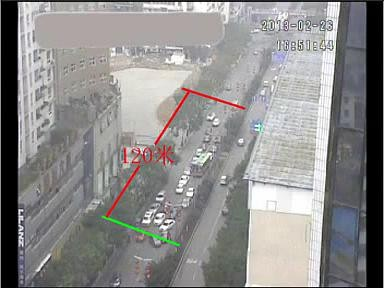
\includegraphics[width=.6\textwidth]{fig1}
%   \caption{发生事故时车流饱和状态图示}
%   \end{figure}

\begin{thebibliography}{10}
% \bibitem{1} \url{http://bbs.chinatex.org}
% \bibitem{2} \url{http://www.chinatex.org}
% \bibitem{3} Alpha Huang, \textbf{latex-notes-zh-cn}, 2014.
% \bibitem{lf}M.R.C. van Dongen,\textbf{\LaTeX-and-Friends}, 2013.
% \bibitem{figure}Keith Reckdahl,\textbf{Using Import graphics in \LaTeXe}, 1997.
% \bibitem{HM}Addison Wesley,\textbf{Higher Mathematics}, 下载地址如下\\ \url{http://media.cism.it/attachments/ch8.pdf}
\end{thebibliography}


\newpage
\appendix
\section*{附 \quad 录}

\subsection{MATLAB源代码}

\begin{verbatim}
clc, clear all


% 读取文件
% 如要修改,将***.xlsx文件路径填入,或者放在此m文件相同目录下,使用xlsread('***.xlsx')
data1 = xlsread('D:\Mcm\Test1\上行上下车.xlsx');
data2 = xlsread('D:\Mcm\Test1\下行上下车.xlsx');

% 上行为1,下行为2
% 上车下车人数分别存储在矩阵 up 和 down 中
for i = 1:2:36
    up1((i+1)/2,:) = data1(i,:);
end
for i = 2:2:36
    down1(i/2,:) = data1(i,:);
end

for i = 1:2:36
    up2((i+1)/2,:) = data2(i,:);
end
for i = 2:2:36
    down2(i/2,:) = data2(i,:);
end

% 每站上车人数与下车人数之差
A1 = up1 - down1;
A2 = up2 - down2;

B1 = max(A1');
B2 = max(A2');

% 每个时间段需要的车辆数下限
m1 = B1 ./ 120;
m2 = B2 ./ 120;

% 车辆数有小数部分处理
m1 = floor(m1 + 1);
m2 = floor(m2 + 1);
% 至少发6辆车
m1(find(m1 < 5)) = 6;
m2(find(m2 < 5)) = 6;

save('m1','m1');
save('m2','m2');
% 寻找一天所要的最少车辆数
max(m1)
max(m2)
%save( 'upHt.met','E');
%save( 'downHt.met','E');

% 每段时间的发车时间间隔
Dt1 = 60 ./ m1;
Dt2 = 60 ./ m2;

% 保存
save('Dt1','Dt1');
save('Dt2','Dt2');




`clc, clear all


% 读取文件
data1 = xlsread('D:\Mcm\Test1\上行各站距离.xlsx');
data2 = xlsread('D:\Mcm\Test1\下行各站距离.xlsx');

t1 = data1 ./ (20 ./ 60)
t2 = data2 ./ (20 ./ 60)

T1 = sum(t1)
T2 = sum(t2)

clc,clear all

load('m1')
load('m2')
load('Dt1')
load('Dt2')

temp1 = 0;
for i = 1:length(Dt1)
    num1(i) = 60 ./ floor(Dt1(i));
    if isinteger(num1(i))
    else num1(i) = round(num1(i));
    end
    temp1 = (60 + temp1) - num1(i) .* Dt1(i);
end

temp2 = 0;
for i = 1:length(Dt1)
    num2(i) = 60 ./ floor(Dt2(i));
    if isinteger(num2(i))
    else num2(i) = round(num2(i));
    end
    temp2 = (60 + temp2) - num2(i) .* Dt2(i);
end

num1
num2


\end{verbatim}

\end{document}
